\documentclass[../main.tex]{subfiles}
\graphicspath{{\subfix{../images/}}}
\begin{document}
\section*{Introduction}
While the natural numbers, integers and rational numbers have a mostly standard construction, the real numbers do not. In \textit{The real numbers - a survey of constructions}~\cite{Weiss2015} Weiss listed 19 (!) constructions of the real numbers. According to the paper these were most, if not all, constructions known at that time (2015). This increase in the ways the real numbers can be constructed in a way reflects their important distinction from the rational numbers. It is also evidence that their construction is likely not as straightforward as the constructions of the other number systems were. This is then also what makes their construction particularly interesting.

We will give three constructions. The first two constructions are the earliest and also most common formal constructions. They both date back to 1872. They are similar in nature, as they both lead to a central concept in the characterisation of the real numbers: completeness. The fact that the rational numbers seem to be incomplete dates back to as early as Ancient Greece. Completeness is what will distinguish the real numbers from the rational numbers. Intuitively a space is complete when it no longer has any holes. What these holes are precisely is dependent on the notion of completeness that is induced by the construction. Briefly put, by making an observation about something that does not hold in the rational numbers, the real numbers are constructed by addressing this deficiency.

The third construction is special. It is much more recent, and has an entirely different approach. Here the the focus is not so much on what properties the rational numbers lack, but on how the real numbers can be viewed. In fact, the rational numbers are skipped over entirely; the real numbers will be directly built from the integers.

Especially in the first two constructions, we will appeal to our intuition of what the real numbers should satisfy. Based on these intuitions, we will prove certain properties for each construction. This ensures that what we are constructing also aligns with what we want to construct.

In Section~\ref{sec:the_real_numbers:dedekinds_construction} we will give the first construction, the construction by Dede\-kind. In Section~\ref{sec:the_real_numbers:cantors_construction} we will walk through Cantor's construction. The last construction, by Schanuel, will be covered in Section~\ref{sec:the_real_numbers:schanuels_construction}. Their equivalence will be proven in Section~\ref{sec:the_real_numbers:uniqueness_of_R}. We will do this by showing they all satisfy a particular characterisation of the real numbers. A comparison of the constructions will be given in Section~\ref{sec:the_real_numbers:comparison_of_the_constructions}. We will end with some closing remarks and possibilities for further research in Section~\ref{sec:the_real_numbers:further_research}.

\section{Dedekind's construction}\label{sec:the_real_numbers:dedekinds_construction}
Dedekind observed the following about the rational numbers he denoted $R$~\cite{Dedekind1872}:
\begin{quote}
    \textgerman{Ist $a$ eine bestimmte Zahl, so zerfallen alle Zahlen des Systems $R$ in zwei Klassen, $A_1$ und $A_2$, deren jede unendlich viele Individuen enthält; die erste Klasse $A_1$ umfaßt alle Zahlen $a_1$, welche $<a$ sind, die zweite Klasse $A_2$ umfaßt alle Zahlen $a_2$, welche $>a$ sind; [\dots].}
\end{quote}
\begin{quote}
    \textit{If $a$ is a certain number, then all numbers in the system $R$ fall into two classes, $A_1$ and $A_2$, each of which contains infinitely many individuals; the first class $A_1$ includes all numbers $a_1$ which are $<a$, the second class $A_2$ includes all numbers $a_2$ which are $>a$; [\ldots].}
\end{quote}
He called such a division a ``\textgerman{Schnitte}'' (cut). Curiously, Dedekind did not come up with this idea himself. He was inspired by Euclid, who wrote the following in Definition~5 of Book~V of \textit{Elements} over two millennia earlier~\cite{Heath1926}!
\begin{quote}
    \textgreek{Ἐν τῷ αὐτῷ λόγῳ μεγέθη λέγεται εἶναι πρῶτον πρὸς δεύτερον καὶ τρίτον πρὸς τέταρτον, ὅταν τὰ τοῦ πρώτου καὶ τρίτου ἰσάκις πολλαπλάσια τῶν τοῦ δευτέρου καὶ τετάρτου ἰσάκις πολλαπλασίων καθ᾽ ὁποιονοῦν πολλαπλασιασμὸν ἑκάτερον ἑκατέρου ἢ ἅμα ὑπερέχῃ ἢ ἅμα ἴσα ἢ ἅμα ἐλλείπῃ ληφθέντα κατάλληλα.}
\end{quote}
\begin{quote}
    \textit{Magnitudes are said to be in the same ratio, the first to the second and the third to the fourth, when, if any equimultiples whatever are taken of the first and third, and any equimultiples whatever of the second and fourth, the former equimultiples alike exceed, are alike equal to, or alike fall short of, the latter equimultiples respectively taken in corresponding order.}
\end{quote}
That is, a ratio of two numbers (here to be understood as a rational number) is defined by the three classes of rational numbers it produces; those less than it, equal to it, and greater than it. Euclid himself took this from Eudoxus' theory of proportions. Even though the necessary mathematics were not there yet for Euclid to construct the real numbers, the ideas were long present. To actually construct the real numbers, Dedekind importantly noted the following:
\begin{quote}
    \textgerman{Aber man überzeugt sich leicht, daß auch unendlich viele Schnitte existieren, welche nicht durch rationale Zahlen hervorgebracht werden.}
\end{quote}
\begin{quote}
    \textit{But one can easily convince oneself that there are also infinitely many cuts which are not produced by rational numbers.}
\end{quote}
He gives the following example. Let $D$ be a positive integer that is not the square of an integer. Then there exists a positive integer $\lambda$ such that
\begin{equation*}
    \lambda^2<D<(\lambda+1)^2.
\end{equation*}
He then continues to prove that the cut defined by the squares of rational numbers less than $D$ and greater than $D$ is not produced by any rational number. Dedekind observed that, contrary to the rational numbers, the real numbers do intuitively have the property that every cut is produced by a real number. It was this insight, which Dedekind deemed trivial
\begin{quote}
    \textgerman{Wie schon gesagt, glaube ich nicht zu irren, wenn ich annehme, daß jedermann die Wahrheit dieser Behauptung sofort zugeben wird; die meisten meiner Leser werden sehr enttäuscht sein, zu vernehmen, daß durch diese Trivialität das Geheimnis der Stetigkeit enthüllt sein soll.}
\end{quote}
\begin{quote}
    \textit{As I have already said, I do not think I am mistaken in assuming that everyone will immediately admit the truth of this statement; most of my readers will be very disappointed to hear that the secret of continuity is revealed by this triviality.}
\end{quote}
that revealed the ``\textgerman{Geheimnis der Stetigkeit}'' (secret of continuity). To start, we will first give the following definition.
\begin{definition}[Partition]
    A partition $\mathcal{F}$ of a set $X$ is a family of subsets of $X$ such that
    \begin{itemize}
        \item $\varnothing\notin\mathcal{F}$,
        \item $\bigcup\mathcal{F}=X$,
        \item $\forall A\in\mathcal{F}\forall B\in\mathcal{F}(A\neq B\implies A\cap B=\varnothing)$.
    \end{itemize}
\end{definition}
The cuts, now to be called Dedekind cuts, can then be defined as follows.
\begin{definition}[Dedekind cut]
    A Dedekind cut of $\bbQ$ is a partition into two subsets $(A,B)$ of $\bbQ$ such that $A$ is closed downwards
    \begin{equation*}
        \forall q\in A\forall p\in\bbQ(p<q\implies p\in A),
    \end{equation*}
    $B$ is closed upwards
    \begin{equation*}
        \forall q\in B\forall p\in\bbQ(p>q\implies p\in B)
    \end{equation*}
    and $A$ does not contain a greatest element
    \begin{equation*}
        \forall p\in A\exists q\in A(q>p).
    \end{equation*}
\end{definition}
\begin{figure}[!htbp]
    \centering
    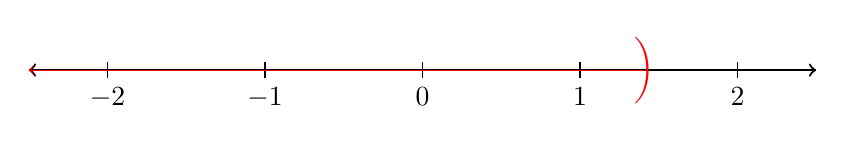
\begin{tikzpicture}
    \draw[thick, <->] (-5, 0) -- (5, 0);

    \draw (0, 0.1) -- (0, -0.1) node[anchor=north] {$0$};
    \draw (2, 0.1) -- (2, -0.1) node[anchor=north] {$1$};
    \draw (4, 0.1) -- (4, -0.1) node[anchor=north] {$2$};
    \draw (-2, 0.1) -- (-2, -0.1) node[anchor=north] {$-1$};
    \draw (-4, 0.1) -- (-4, -0.1) node[anchor=north] {$-2$};

    \draw[red] (2.828, 0) node[anchor=center] {$\biggr)$};
    \draw[red, <-] (-5, 0) -- (2.828, 0);
\end{tikzpicture}

    \caption{The Dedekind cut $\{q\in\bbQ\mid q<0\lor q\cdot q<2\}$}
    \label{fig:the_real_numbers:dedekind_cut}
\end{figure}
Figure~\ref{fig:the_real_numbers:dedekind_cut} is an example of a Dedekind cut. Hence intuitively, the cuts are of the form ``$(-\infty,a)$'' so that every element of $A$ is less than every element in $B$. Notice that $A$ being closed downloads implies $B$ is closed upwards. This means that for a partition $(A,B)$ being a Dedekind cut only imposes restrictions on the first set $A$. The set $B$ is then completely determined by $A$. We can therefore uniquely identify the partition $(A,B)$ by its first component $A$. With this, we can define the real numbers as the set of all Dedekind cuts.
\begin{definition}[Real numbers]
    Define the set $\bbR_D$ of (Dedekind) real numbers by
    \begin{equation*}
        \bbR_D\coloneq\{A\in\mathcal{P}(\bbQ)\mid A\text{ is a Dedekind cut of }\bbQ\}.
    \end{equation*}
\end{definition}
Most operations on the Dedekind cuts are easy to define, like addition.
\begin{definition}[Addition of real numbers]
    Define addition as the map $\bbR_D\times\bbR_D\to\bbR_D$ defined by
    \begin{equation*}
        A+B=\{a+b\in\bbQ\mid a\in A\land b\in B\}.
    \end{equation*}
\end{definition}
One can verify that $A+B$ is again a Dedekind cut.
\begin{proposition}\label{prp:the_real_numbers:dedekind_abelian_group_real_numbers}
    $(\bbR_D,+)$ is an abelian group.
\end{proposition}
\begin{proof}
    We will prove each requirement.
    \begin{description}
        \item[Commutative.] Let $A\in\bbR_D$ and $B\in\bbR_D$ be arbitrary. We have
        \begin{align*}
            A+B & =\{a+b\in\bbQ\mid a\in A\land b\in B\} \\
            & =\{b+a\in\bbQ\mid b\in B\land a\in A\}=B+A.
        \end{align*}
        \item[Identity.] Define $0\coloneq\{q\in\bbQ\mid q<0\}$. Then $0$ is a Dedekind cut. Further we need to show that
        \begin{equation*}
            A+0=\{a+q\in\bbQ\mid a\in A\land q<0\}
        \end{equation*}
        is equal to $A$. It is clear that $A\subseteq A+0$. Let $a+q\in\bbQ$ with $a\in A$ and $q<0$ be arbitrary. Because $A$ is closed downwards we have that since $a+q<a$ we also have $a+q\in A$. We conclude $A+0=A$.
        \item[Associative.] Let $A\in\bbR_D$, $B\in\bbR_D$ and $C\in\bbR_D$ be arbitrary. Then
        \begin{align*}
            A+(B+C) & =A+\{b+c\in\bbQ\mid b\in B\land c\in C\} \\
            & =\{a+x\in\bbQ\mid a\in A\land x\in\{b+c\in\bbQ\mid b\in B\land c\in C\}\} \\
            & =\{a+(b+c)\in\bbQ\mid a\in A\land b\in B\land c\in C\} \\
            & =\{(a+b)+c\in\bbQ\mid a\in A\land b\in B\land c\in C\} \\
            & =\{x+c\in\bbQ\mid x\in\{a+b\in\bbQ\mid a\in A\land b\in B\}\land c\in C\} \\
            & =\{a+b\in\bbQ\mid a\in A\land b\in B\}+C \\
            & =(A+B)+C.
        \end{align*}
        \item[Inverse.] Let $A\in\bbR_D$ be arbitrary. Take $-A\coloneq\{q-b\in\bbQ\mid q<0\land b\in\bbQ\setminus A\}$. Then $-A$ is a Dedekind cut and
        \begin{align*}
            A+(-A) & =\{a+(q-b)\in\bbQ\mid q<0\land a\in A\land b\in\bbQ\setminus A\} \\
            & =\{q+(a-b)\in\bbQ\mid q<0\land a\in A\land b\in\bbQ\setminus A\} \\
            & =\{q+p\in\bbQ\mid q<0\land p<0\} \\
            & =\{q\in\bbQ\mid q<0\}=0.
        \end{align*}
    \end{description}
\end{proof}
Unfortunately, multiplication is slightly harder to define. A naive definition would be $A\cdot B=\{a\cdot b\in\bbQ\mid a\in A\land b\in B\}$. Recall that intuitively the cuts are of the form ``$(-\infty,a)$''. We would for example want that ``$(-\infty,-1)\cdot(-\infty,-1)=(-\infty,1)$''. With this definition however, since $-2$ is in both intervals, $-2\cdot-2=4$ would be in the resulting interval. We therefore need to ignore the negative numbers and add them back in manually. We also need to consider the sign of both numbers in separate cases. For this reason, we will first define the order on the real numbers. Luckily this is very straightforward.
\begin{definition}[Order on real numbers]
    Define the order on $\bbR_D$ as $A\leq B$ if $A\subseteq B$.
\end{definition}
We want to define multiplication for negative real numbers in terms of multiplication of nonnegative real numbers. That means we need the fact that if $A<0$ then $-A>0$. We will thus prove that $\leq$ is a total order and that the order is preserved under addition.
\begin{proposition}\label{prp:the_real_numbers:dedekind_totally_ordered_abelian_group_real_numbers}
    $(\bbR_D,+,\leq)$ is an ordered abelian group.
\end{proposition}
\begin{proof}
    By Proposition~\ref{prp:the_real_numbers:dedekind_abelian_group_real_numbers} we know that $(\bbR_D,+)$ is an abelian group. It remains to show that $(\bbR_D,\leq)$ is a total order and that the order is preserved under addition. Transitivity follows by transitivity of $\subseteq$ and antisymmetry follows directly by the \nameref{subsec:zermelo_fraenkel_set_theory:axiom_of_extensionality}.
    \begin{description}
        \item[Strongly connected.] By way of contradiction, suppose $A\not\leq B$ and $B\not\leq A$. Then there exists an $a\in A$ such that $a\notin B$ and a $b\in B$ such that $b\notin A$. By strongly connectedness of $\bbQ$, we may without loss of generality assume $a<b$. Since $B$ is closed downwards we must have $a\in B$, a contradiction.
        \item[OR1.] Let $A\in\bbR_D$, $B\in\bbR_D$ and $C\in\bbR_D$ be arbitrary and suppose $A\leq B$. We want to show that $A+C\leq B+C$. Let $a+c\in A+C$ be arbitrary. Since $A\subseteq B$ we know $a\in B$. Hence $a+c\in B+C$.
    \end{description}
\end{proof}
If we now have $A<0$, we see that $-A>0$ by adding $-A$ to both sides. Now we can define multiplication.
\begin{definition}[Multiplication of real numbers]
    Define multiplication as the map $\bbR_D\times\bbR_D\to\bbR_D$ defined by
    \begin{equation*}
        A\cdot B=
        \begin{cases}
            \{a\cdot b\in\bbQ\mid a\in A\land a\geq0\land b\in B\land b\geq0\}\cup0 & \text{if }A\geq0\land B\geq0 \\
            -((-A)\cdot B) & \text{if }A<0\land B\geq0 \\
            -(A\cdot(-B)) & \text{if }A\geq0\land B<0 \\
            (-A)\cdot(-B) & \text{if }A<0\land B<0
        \end{cases}.
    \end{equation*}
\end{definition}
It can be verified that $A\cdot B$ is a Dedekind cut. $\bbR_D$ has the following structure.
\begin{proposition}\label{prp:the_real_numbers:dedekind_ordered_field_real_numbers}
    $(\bbR_D,+,\cdot,\leq)$ is an ordered field.
\end{proposition}
\begin{proof}
    By Proposition~\ref{prp:the_real_numbers:dedekind_totally_ordered_abelian_group_real_numbers} we know that $(\bbR_D,+,\leq)$ is a totally ordered abelian group. It remains to show that $(\bbR_D,+,\cdot)$ is a field and that the order is preserved under multiplication. Throughout the proof we will assume all real numbers to be nonnegative. The cases for negative values are similar. Denote $\bbR_D^{\geq0}=\{A\in\bbR_D\mid A\geq0\}$. The proofs for associativity and distributivity are omitted.
    \begin{description}
        \item[Commutative.] Let $A\in\bbR_D^{\geq0}$ and $B\in\bbR_D^{\geq0}$ be arbitrary. We want to show that $A\cdot B=B\cdot A$. We have
        \begin{align*}
            A\cdot B & =\{a\cdot b\in\bbQ\mid a\in A\land a\geq0\land b\in B\land b\geq0\}\cup0 \\
            & =\{b\cdot a\in\bbQ\mid b\in B\land b\geq0\land a\in A\land a\geq0\}\cup0=B\cdot A.
        \end{align*}
        \item[Identity.] Define $1\coloneq\{q\in\bbQ\mid q<1\}$. Then $1$ is a Dedekind cut. Let $A\in\bbR_D^{\geq0}$ be arbitrary. We have
        \begin{align*}
            A\cdot1 & =\{a\cdot q\in\bbQ\mid a\in A\land a\geq0\land q<1\land q\geq0\}\cup0 \\
            & =\{a\in\bbQ\mid a\in A\land a\geq0\}\cup0 \\
            & =\{a\in\bbQ\mid a\in A\}=A,
        \end{align*}
        where we used that multiplying $a$ by $0\leq q<1$ cannot result in $a$ leaving $A$ or $a<0$.
        \item[Inverse.] Let $A\in\bbR_D$ be arbitrary with $A>0$. Define $A^{-1}\coloneq\{q/b\in\bbQ\mid q<1\land b\in\bbQ\setminus A\}$. Then
        \begin{align*}
            A\cdot A^{-1} & =\{a\cdot(q/b)\in\bbQ\mid a\in A\land a\geq0\land q<1\land b\in\bbQ\setminus A\land q\geq0\}\cup0 \\
            & =\{q\cdot(a/b)\in\bbQ\mid a\in A\land a\geq0\land q<1\land b\in\bbQ\setminus A\land q\geq0\}\cup0 \\
            & =\{q\cdot p\in\bbQ\mid q<1\land q\geq0\land p<1\land p\geq0\}\cup0 \\
            & =\{q\in\bbQ\mid q<1\land q\geq0\}\cup0 \\
            & =\{q\in\bbQ\mid q<1\}=1,
        \end{align*}
        where we used that multiplying $q$ by $0\leq a/b<1$ cannot result in $q>1$ or $q<0$.
        \item[OR2.] Let $A\in\bbR_D^{\geq0}$, $B\in\bbR_D^{\geq0}$ and $C\in\bbR_D^{\geq0}$ with $A\leq B$ be arbitrary. We wish to show that $A\cdot C\leq B\cdot C$. Let $a\cdot c\in A\cdot C$ be arbitrary. Then $a\in B$ as $A\subseteq B$. Hence $A\cdot C\leq B\cdot C$.
    \end{description}
\end{proof}
We just showed that $\bbR_D$ is an ordered field. In Proposition~\ref{prp:the_natural_numbers_integers_and_rational_numbers:ordered_field_rational_numbers} we saw that $\bbQ$ also has this structure. However, $\bbR_D$ has an important property $\bbQ$ does not have. That is, $\bbQ$ has Dedekind cuts that are not produced by rational numbers. Since we constructed $\bbR_D$ by filling these holes, we expect that $\bbR_D$ no longer has any. This is indeed the case, and is known as Dedekind-completeness. This is the secret of continuity Dedekind alluded to. 
\begin{proposition}[$\bbR_D$ is Dedekind-complete]\label{prp:the_real_numbers:dedekind_R_dedekind_complete}
    For every Dedekind cut $A$ of $\bbR_D$ there exists an $x\in\bbR_D$ such that $A=\{a\in\bbR_D\mid a<x\}$.
\end{proposition}
\begin{proof}
    Let $A$ be a Dedekind cut of $\bbR_D$. Define $x=\bigcup A$. Then $x$ is the result of combining all Dedekind cuts that exist in $A$. We claim that $A=\{a\in\bbR_D\mid a<x\}$. To show $x\in\bbR_D$ we need to show that $x$ is a Dedekind cut of $\bbQ$. Clearly $x$ is nonempty and not equal to $\bbQ$. To show that $x$ is closed downwards, suppose $p<q$ for any $q\in x$ and $p\in\bbQ$. Since $q\in x$ we have that there exists an $a\in A$ such that $q\in a$. Since $a$ is closed downwards we must have $p\in a$ and hence $p\in x$. By a similar argument $x$ does not contain a greatest element. Next we will show $A\subseteq\{a\in\bbR_D\mid a<x\}$. Let $a\in A$ be arbitrary. Since we have $a\subseteq x$, by definition also $a\leq x$. And since $A$ has no greatest element, there exists a $b\in A$ such that $a<b\leq x$. Thus $a\neq x$. Lastly we will show $\{a\in\bbR_D\mid a<x\}\subseteq A$. Let $a\in\bbR_D$ with $a<x$ be arbitrary. Take $p\in x\setminus a$. Then we have $a\subseteq\{q\in\bbQ\mid q<p\}$. If we now take $b\in A$ with $p\in b$, we find $a\subseteq\{q\in\bbQ\mid q<p\}\subseteq b$ and hence $a\in A$.
\end{proof}
Instead of Dedekind-completeness, in the literature one often refers to this property as the least-upper-bound property of the real numbers. This equivalent property is more practical, whereas the Dedekind-completeness property is more instructional. To state the least-upper-bound property, we will first state two definitions on which it depends.
\begin{definition}[Bounded (above) set]
    Let $(X,\leq)$ be a total order. Let $A\subseteq X$ be a subset of $X$. Then $A$ is bounded if $\exists S\in X\forall x\in A(\vert x\vert\leq S)$ and bounded above if $\exists S\in X\forall x\in A(x\leq S)$. We say that $A$ is unbounded (above) when it is not bounded (above).
\end{definition}
\begin{definition}[Supremum]\label{dfn:the_real_numbers:supremum}
    Let $(X,\leq)$ be a total order. Let $A\subseteq X$ be a subset of $X$. Then $S\in X$ is a supremum of $A$ if
    \begin{itemize}
        \item $\forall x\in A(x\leq S)$,
        \item $\forall T\in X((\forall x\in A(x\leq T))\implies S\leq T)$.
    \end{itemize}
    By the antisymmetry of the order it quickly follows that the supremum is unique.
\end{definition}
The first requirement of Definition~\ref{dfn:the_real_numbers:supremum} is that the supremum is an upper bound, the second is that it is the least upper bound; it is less than or equal to all other upper bounds. The least-upper-bound property can be stated as follows.
\begin{definition}[Least-upper-bound property]
    An ordered field $\bbK$ satisfies the least-upper-bound property when every bounded above subset of $\bbK$ has a supremum.
\end{definition}
We will now prove Dedekind-completeness and the least-upper-bound property are in fact equivalent.
\begin{proposition}\label{prp:the_real_numbers:characterisation_dedekind_complete}
    Let $\bbK$ be an ordered field. Then $\bbK$ is Dedekind-complete if and only if $\bbK$ satisfies the least-upper-bound property.
\end{proposition}
\begin{proof}
    Suppose $\bbK$ is Dedekind-complete. Let $A$ be a bounded above subset of $\bbK$. If $A$ has a maximum $M$, then it is clear it is also the supremum. Therefore suppose $A$ has no greatest element. Define $B=\bigcup\{\{b\in\bbK\mid b<a\}\in\mathcal{P}(\bbK)\mid a\in A\}$. It is routine to verify that $B$ is a Dedekind cut. Hence there exists an $S\in\bbK$ such that $B=\{b\in\bbK\mid b<S\}$. We will show that $S$ is the supremum of $A$. Let $a\in A$ be arbitrary. Since $A$ has no greatest element, there is a $b\in A$ such that $b>a$. Since $\{c\in\bbK\mid c<b\}\subseteq B$, we have $a\in B$ and so $a<S$. Let $T$ be another upper bound of $A$ and by way of contradiction suppose $T<S$. Then $T\in B$. Hence there exists an $a\in A$ such that $T\in\{c\in\bbK\mid c<a\}$, so $T<a$. This contradicts that $T$ is an upper bound of $A$.

    Now suppose $\bbK$ satisfies the least-upper-bound property. Let $A$ be a Dede\-kind cut of $A$. Then $A$ is clearly bounded above, so there exists a supremum $S$ of $A$. We will prove that $A=\{a\in\bbK\mid a<S\}$. Let $a\in A$ be arbitrary. Because $A$ has no greatest element, we have $S\notin A$. Hence $a<S$ because $S$ is an upper bound of $A$. Now let $a\in\bbK$ with $a<S$ be arbitrary. Then $a$ is not an upper bound of $A$, so there exists a $b\in A$ for which $b>a$. Because $A$ is closed downwards we find $a\in A$.
\end{proof}
By Theorem~\ref{thm:the_natural_numbers_integers_and_rational_numbers:Q_smallest_ordered_field} there exists an embedding from $\bbQ$ to $\bbR_D$. Even though we gave a constructive proof, it is practical to state the embedding explicitly. The embedding is given by $f:\bbQ\to\bbR_D$ defined by $f(q)=\{a\in\bbQ\mid a<q\}$. It can be readily verified $f$ is indeed an embedding.

\section{Cantor's construction}\label{sec:the_real_numbers:cantors_construction}
The next construction, usually attributed to Cantor\footnote{It is actually due to Méray, who published his work three years earlier~\cite{Meray1869}.}, uses a certain sense of closeness of members of a sequence. In his own words~\cite{Cantor1883}:
\begin{quote}
    \textgerman{[\dots] ich fordre, dass nach Annahme einer beliebig kleinen rationalen Zahl $\epsilon$ eine endliche Anzahl von Gliedern der Menge abgeschieden werden kann, so dass die übrig bleibenden paarweise einen Unterschied haben, der seiner absoluten Grösse nach kleiner ist als $\epsilon$.}
\end{quote}
\begin{quote}
    \textit{[\ldots] I require that after assuming an arbitrarily small rational number $\epsilon$, a finite number of members of the set can be separated so that the remaining pairs have a difference that is smaller in absolute size than $\epsilon$.}
\end{quote}
This notion of closeness may be familiar to the reader. Today sequences with this property are called Cauchy sequences. Cantor used these Cauchy sequences (or ``\textgerman{Fundamentalreihe}'' as he called them) to construct the real numbers. See Figure~\ref{fig:the_real_numbers:cauchy_sequence} for an example of a Cauchy sequence\footnote{Decimal expansions are also Cauchy sequences but are hard to define for irrational numbers without prior knowledge of them.}.
\begin{figure}[!htbp]
    \centering
    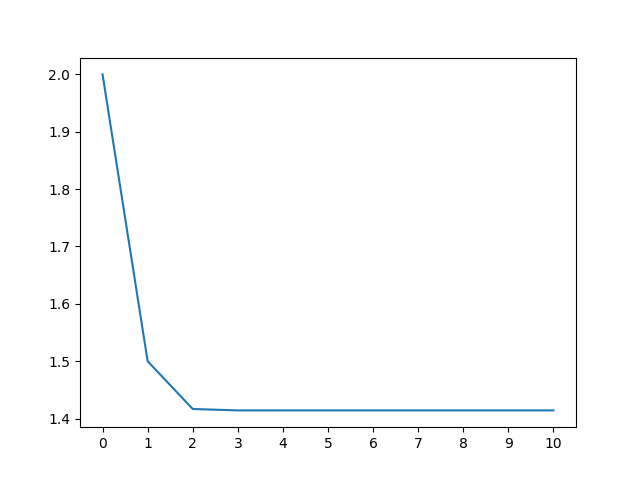
\includegraphics[width=0.75\linewidth]{figures/cauchy_sequence}
    \caption{The Cauchy sequence $(q_n):\bbN\to\bbQ$ defined by $q_0=2$ and $q_{n+1}=(q_n+2/q_n)/2$}
    \label{fig:the_real_numbers:cauchy_sequence}
\end{figure}

With ``\textgerman{absoluten Grösse}'' (absolute in size) Cantor meant that the sign of a number is unimportant; only its magnitude is. For this, we will introduce a new function.
\begin{definition}[Absolute value function]\label{dfn:the_real_numbers:absolute_value_function}
    We define the absolute value function as the map $\bbQ\to\{q\in\bbQ\mid q\geq0\}$ defined by
    \begin{equation*}
        \vert q\vert=
        \begin{cases}
            q & \text{if }q\geq0 \\
            -q & \text{if }q<0
        \end{cases}.
    \end{equation*}
\end{definition}
Cantor considered Cauchy sequences of rational numbers. For a given Cauchy sequence, he stated that ``\textgerman{Der Reihe hat eine bestimmte Grenze $b$}'' (the sequence has a certain limit $b$)~\cite{Cantor1872}. That is, since a Cauchy sequence is a sequence for which its values get closer and closer together, Cantor argued it must have a limit. These limits are precisely the real numbers. This however, is slightly inaccurate. To see why, we will now formally state what it means for a sequence to be Cauchy, and to have a limit (to converge).
\begin{definition}[Cauchy sequence]
    A sequence $(q_n):\bbN\to\bbQ$ is Cauchy if
    \begin{equation*}
        \forall\epsilon>0_\bbQ\exists N\in\bbN\forall m\geq N\forall n\geq N(\vert q_m-q_n\vert<\epsilon).
    \end{equation*}
\end{definition}
\begin{definition}[Convergent sequence]
    A sequence $(q_n):\bbN\to\bbQ$ is convergent if
    \begin{equation*}
        \exists q\in\bbQ\forall\epsilon>0_\bbQ\exists N\in\bbN\forall n\geq N(\vert q_n-q\vert<\epsilon),
    \end{equation*}
    in which case we write $q_n\to q$.
\end{definition}
Crucially convergence of a rational sequence requires the existence of a rational number to which it converges; its limit. Cauchy sequences do not require this. But if every rational Cauchy sequence has a limit (it converges), it too must be a rational number. That is, we would not have constructed the real numbers at all. That must mean that not every rational Cauchy sequence converges. This is indeed the case. In particular, the Cauchy sequences that do not converge, reveal ``holes'' in the rational numbers. These holes are precisely the irrational numbers; the real numbers which are not rational. In particular, the Cauchy sequence from Figure~\ref{fig:the_real_numbers:cauchy_sequence} is not convergent.

Since the Cauchy sequences reveal the gaps in the rational numbers, the Cauchy sequences are what will represent the real numbers. Note that more than one Cauchy sequence can represent a single real number, though. A trivial case of this is when the first term in a sequence is changed to an arbitrary other rational number. This will not affect the Cauchy property a sequence has. For this reason, we will have to define a relation on these Cauchy sequences and unify them in equivalence classes. We will do this as follows. Define the relation $\sim$ on $C_\bbQ\coloneq\{(q_n)\in\bbQ^\bbN\mid(q_n)\text{ is Cauchy}\}$ by
\begin{equation}\label{eqn:the_real_numbers:cantor_relation_real_numbers}
    (p_n)\sim(q_n)\iff\vert p_n-q_n\vert\to0.
\end{equation}
Two Cauchy sequences are related when the sequence defined by the absolute value of their difference converges to $0$. This allows us to unify the Cauchy sequences that approximate the same real number.
\begin{lemma}
    The relation $\sim$ as defined in Equation~\eqref{eqn:the_real_numbers:cantor_relation_real_numbers} is an equivalence relation.
\end{lemma}
\begin{proof}
    Reflexivity and symmetry follow quite directly. Transitivity follows from the triangle inequality, which we will assume the reader is familiar with.
\end{proof}
As such, we will now define the real numbers as the equivalence classes of $\sim$.
\begin{definition}[Real numbers]
    Define the set $\bbR_C$ of (Cantor) real numbers by $\bbR_C\coloneq C_\bbQ/{\sim}$.
\end{definition}
Part of the elegance of this construction is that all operations work pointwise.
\begin{definition}[Addition of real numbers]
    Define addition as the map $\bbR_C\times\bbR_C\to\bbR_C$ defined by
    \begin{equation*}
        [(p_n)]+[(q_n)]=[(p_n+q_n)].
    \end{equation*}
\end{definition}
\begin{definition}[Multiplication of real numbers]
    Define multiplication as the map $\bbR_C\times\bbR_C\to\bbR_C$ defined by
    \begin{equation*}
        [(p_n)]\cdot[(q_n)]=[(p_n\cdot q_n)].
    \end{equation*}
\end{definition}
One should verify that both these functions are well-defined, and in particular that when $(p_n)$ and $(q_n)$ are Cauchy sequences, then so are $(p_n+q_n)$ and $(p_n\cdot q_n)$. Because the operations work pointwise, the properties of addition and multiplication are mostly immediate from their properties on $\bbQ$.
\begin{proposition}\label{prp:the_real_numbers:cantor_field_real_numbers}
    $(\bbR_C,+,\cdot)$ is a field.
\end{proposition}
\begin{proof}
    Most properties follow directly by the properties on the rational numbers as shown in Proposition~\ref{prp:the_natural_numbers_integers_and_rational_numbers:field_rational_numbers}. The additive identity is $0\coloneq[(0)]$ as for any $[(q_n)]\in\bbR_C$ we have $[(q_n)]+[(0)]=[(q_n+0)]=[(q_n)]$. The additive inverse is $-[(q_n)]\coloneq[(-q_n)]$ as $[(q_n)]+[(-q_n)]=[(q_n-q_n)]=[(0)]=0$. The multiplicative identity is $1\coloneq[(1)]$ as $[(q_n)]\cdot[(1)]=[(q_n\cdot1)]=[(q_n)]$. We need to be a little bit careful for the the multiplicative inverse. We would want to say that it is $[(q_n)]^{-1}\coloneq[(q_n^{-1})]$. However, we might have that $q_n=0$ for various $n\in\bbN$. Furthermore, $(q_n^{-1})$ might not be Cauchy for general $(q_n)$. We will show that when $q_n\not\to0$, there exists an $N\in\bbN$ such that for all $n\geq N$ we have $q_n\neq0$, and moreover that $(q_n^{-1})$ is then Cauchy. Because $q_n\not\to0$, there exists an $\epsilon>0$ such that for all $m\in\bbN$ there exists an $n\geq m$ for which $\vert q_n\vert>\epsilon$. Because $(q_n)$ is Cauchy, there exists an $N\in\bbN$ such that for all $m\geq N$ we have $\vert q_n-q_m\vert<\epsilon/2$. Then $-\epsilon/2<q_n-q_m<\epsilon/2$ so that $-\epsilon/2+q_m<q_n<\epsilon/2+q_m$. Hence $\epsilon<\vert q_n\vert<\epsilon/2+\vert q_m\vert$, so $\vert q_m\vert>\epsilon/2>0$. We will now show $(q_n^{-1})$ is Cauchy. Like before, take $\epsilon>0$ and for any $N\in\bbN$ take $n\geq N$ for which $\vert q_n\vert>\epsilon$. Because $(q_n)$ is Cauchy, there exists an $N\in\bbN$ such that for $m\geq N$ we have $\vert q_m-q_n\vert<\epsilon\cdot\epsilon\cdot\epsilon$. Without loss of generality suppose $q_m>\epsilon$. Then $\vert1/q_m-1/q_n\vert=\vert q_n-q_m\vert/\vert q_m\cdot q_n\vert<\epsilon\cdot\epsilon\cdot\epsilon/(\epsilon\cdot\epsilon)=\epsilon$. We conclude that for $[(q_n)]\neq0$ we can thus pick a nonzero representative $(q_n)$ to define $[(q_n)]^{-1}=[(q_n^{-1})]$. This is the inverse as $[(q_n)]\cdot[(q_n^{-1})]=[(q_n\cdot q_n^{-1})]=[(1)]=1$.
\end{proof}
The order also works pointwise, but for the tail of the sequence. The first few terms of the sequence need not obey the order, it only matters how the sequence behaves after a certain point.
\begin{definition}[Order on real numbers]\label{dfn:the_real_numbers:cantor_order}
    Define the order on $\bbR_C$ as $[(p_n)]\leq[(q_n)]$ if there exists an $N\in\bbN$ such that for all $n\geq N$ it is true that $p_n\leq q_n$.
\end{definition}
That is, $(p_n)$ is eventually smaller than $(q_n)$. It can be checked that this is well-defined. Before proving $\bbR_C$ is an ordered field, we will give two more usual definitions.
\begin{definition}[Maximum, minimum]
    Let $(X,\leq)$ be a total order. Let $A\subseteq X$ be a subset of $X$. Then $M\in A$ is the maximum of $A$ when $a\leq M$ for all $a\in A$, in which case we write $\max(A)=M$. Similarly $M\in A$ is the minimum when $M\leq a$ for all $a\in A$, in which case we write $\min(A)=M$.
\end{definition}
\begin{proposition}\label{prp:the_real_numbers:cantor_ordered_field_real_numbers}
    $(\bbR_C,+,\cdot,\leq)$ is an ordered field.
\end{proposition}
\begin{proof}
    By Proposition~\ref{prp:the_real_numbers:cantor_field_real_numbers} it remains to show $(\bbR_C,\leq)$ is a total order and that addition and multiplication behave nicely over the order.
    \begin{description}
        \item[Transitive.] Suppose $[(p_n)]\leq[(q_n)]$ and $[(q_n)]\leq[(r_n)]$. Then there exists $N_1\in\bbN$ such that $p_n\leq q_n$ for all $n>N_1$ and $N_2\in\bbN$ such that $q_n\leq r_n$ for all $n>N_2$. Take $N=\max\{N_1,N_2\}$. Then for $n>N$ we have both $p_n\leq q_n$ and $q_n\leq r_n$. By transitivity of the order on rational numbers we have $p_n\leq r_n$.
        \item[Antisymmetric.] Suppose $[(p_n)]\leq[(q_n)]$ and $[(q_n)]\leq[(p_n)]$. Then there exists an $N\in\bbN$ such that for all $n>N$ we have $p_n\leq q_n$ and $q_n\leq p_n$, so $p_n=q_n$.
        \item[Strongly connected.] Suppose $[(p_n)]\neq[(q_n)]$. We need to show that $[(p_n)]<[(q_n)]$ or $[(p_n)]>[(q_n)]$. Since $[(p_n)]\neq[(q_n)]$ we have that there exists an $\epsilon>0$ such that for all $N\in\bbN$ there exists $n\geq N$ for which $\vert p_n-q_n\vert\geq\epsilon$. Since $(p_n)$ and $(q_n)$ are Cauchy, there exists $N\in\bbN$ such that for all $m\geq N$ and $n\geq N$ we have both $\vert p_m-p_n\vert<\epsilon$ and $\vert q_m-q_n\vert<\epsilon$, so $p_n-\epsilon<p_m<p_n+\epsilon$ and $q_m-\epsilon<q_n<q_m+\epsilon$. For this $N$ there exists an $n\geq N$ so that either $p_n-q_n\geq\epsilon$ or $p_n-q_n\geq-\epsilon$. In the first case we find for all $m\geq N$ that $p_m>p_n-\epsilon\geq q_n>q_m-\epsilon>q_m$. Hence $[(p_m)]\geq[(q_m)]$. The other case follows similarly.
        \item[OR1.] Suppose $[(p_n)]\leq[(q_n)]$ and let $[(r_n)]$ be arbitrary. Then there exists an $N\in\bbN$ such that $p_n\leq q_n$ for all $n>N$. For this $N$ we then also have $p_n+r_n\leq q_n+r_n$.
        \item[OR1.] Suppose $[(p_n)]\leq[(q_n)]$ and $[(r_n)]\geq0$. Then there exists an $N_1\in\bbN$ such that $p_n\leq q_n$ for all $n>N_1$. There also exists an $N_2\in\bbN$ such that $r_n\geq0$ for all $n>N_2$. For $N=\max\{N_1,N_2\}$ we then have $p_n+r_n\leq q_n+r_n$.
    \end{description}
\end{proof}
We just showed that $\bbR_C$ is an ordered field. It is clear how the pointwise definitions of all operations made the proofs for the structure of $\bbR_C$ very simple. Thus far, $\bbQ$ has the same structure. However, like with the Dedekind real numbers being Dedekind-complete, we now expect that the Cantor real numbers are Cauchy-complete. That is, every real Cauchy sequence should also be a convergent sequence. 
\begin{proposition}[$\bbR_C$ is Cauchy-complete]\label{prp:the_real_numbers:cantor_R_cauchy_complete}
    Every real Cauchy sequence is a convergent sequence.
\end{proposition}
\begin{proof}
    Let $(x_n):\bbN\to\bbR_C$ be a Cauchy sequence. Then for each $n\in\bbN$, the real number $x_n$ is an equivalence class of sequences itself. That is, we have a sequence of equivalent classes of sequences. We are in the following situation.
    \begin{align}\label{eqn:the_real_numbers:sequence_of_sequences}
        \begin{split}
            x_0 & =[(x_{0,0},x_{0,1},x_{0,2},x_{0,3},x_{0,4},\dots)] \\
            x_1 & =[(x_{1,0},x_{1,1},x_{1,2},x_{1,3},x_{1,4},\dots)] \\
            x_2 & =[(x_{2,0},x_{2,1},x_{2,2},x_{2,3},x_{2,4},\dots)] \\
            x_3 & =[(x_{3,0},x_{3,1},x_{3,2},x_{3,3},x_{3,4},\dots)] \\
            x_4 & =[(x_{4,0},x_{4,1},x_{4,2},x_{4,3},x_{4,4},\dots)] \\
             & \vdotswithin{=}
        \end{split}
    \end{align}
    To show every Cauchy sequence is convergent, we need to find a candidate limit. This limit, being a real number, is then also an equivalence class of Cauchy sequences. We thus need to find a candidate Cauchy sequence. Before we do this, we need to pick the representatives more cleverly. Because we picked arbitrary representatives, we do not have any control over their convergence to show this. Using subsequences we can control the convergence rate with something uniform. Let $s_n=1/n$. Since each $(x_{n,k})$ is Cauchy, there exists a $K\in\bbN$ such that for all $k\geq K$ and $l\geq K$ we have $\vert x_{n,k}-x_{n,l}\vert<s_n/6$. Hence we can take the subsequence $(x_{n,K+k})$ so that for all $k\in\bbN$ and $l\in\bbN$ we have $\vert x_{n,K+k}-x_{n,K+l}\vert<s_n/6$. Notice that $(x_{n,k})\sim(x_{n,K+k})$, so from now on we will assume the representatives have the property that $\vert x_{n,k}-x_{n,l}\vert<s_n/6$ for all $k\in\bbN$ and $l\in\bbN$.

    Since $(x_n)$ is Cauchy, for every $i\in\bbN$ there is an $N_i\in\bbN$ such that for $m\geq N_i$ and $n\geq N_i$ we have
    \begin{align*}
        \vert x_m-x_n\vert & =\left\vert[(x_{m,0},x_{m,1},x_{m,2},\dots)]-[(x_{n,0},x_{n,1},x_{n,2},\dots)]\right\vert \\
        & =\left\vert[(x_{m,0}-x_{n,0},x_{m,1}-x_{n,1},x_{m,2}-x_{n,2},\dots)]\right\vert<s_i/6,
    \end{align*}
    so by unwinding Definition~\ref{dfn:the_real_numbers:cantor_order} there is a $K\in\bbN$ such that for $k\geq K$ we have $\vert x_{m,k}-x_{n,k}\vert<s_i/6$. Further note that we can take $N_i$ so that $N_i>i$ and $N_{i+1}>N_i$ by taking $N_i$ to be the maximum over $i+1$ and $N_j+1$ for all $j<i$. To remove the constraint on $k$, we let $m\in\bbN$ with $m\geq N_i$ and $n\in\bbN$ with $n\geq N_i$ be arbitrary and take $K$ such that for $k\geq K$ we have $\vert x_{m,k}-x_{n,k}\vert<s_i/6$. Then for all $l\in\bbN$ we have
    \begin{align*}
        \vert x_{m,l}-x_{n,l}\vert & \leq\vert x_{m,l}-x_{m,k}\vert+\vert x_{m,k}-x_{n,k}\vert+\vert x_{n,k}-x_{n,l}\vert \\
        & <s_m/6+s_i/6+s_n/6 \\
        & <s_i/6+s_i/6+s_i/6=s_i/2.
    \end{align*}
    Now we are ready to construct the candidate sequence. Define the sequence $(y_i):\bbN\to\bbQ$ by $y_i=x_{N_i,N_i}$. Intuitively, these are diagonal elements in Equation~\eqref{eqn:the_real_numbers:sequence_of_sequences} that are far enough down and to the right such that they are close enough to each other. We will show that $(y_i)$ is Cauchy and in fact $x_n\to x$ for $x=[(y_i)]$. Let $k\in\bbN$ be arbitrary. Then for $i\geq k$ and $j\geq k$ we have
    \begin{align*}
        \vert y_i-y_j\vert & =\vert x_{N_i,N_i}-x_{N_j,N_j}\vert \\
        & \leq\vert x_{N_i,N_i}-x_{N_i,N_j}\vert+\vert x_{N_i,N_j}-x_{N_j,N_j}\vert \\
        & <s_{N_i}/2+s_k/2 \\
        & <s_k/2+s_k/2=s_k.
    \end{align*}
    So $\vert y_i-y_j\vert\to0$ because $s_k\to0$. We have now established that $x\in\bbR_C$. It remains to show that $x_n\to x$. Let $k\in\bbN$ be arbitrary. For $i\geq k$, $n\geq N_i$ and $l\geq N_i$ we have
    \begin{align*}
        \vert x_{n,l}-x_{N_l,N_l}\vert & \leq\vert x_{n,l}-x_{n,N_l}\vert+\vert x_{n,N_l}-x_{N_l,N_l}\vert \\
        & <s_n/2+s_k/2 \\
        & \leq s_k/2+s_k/2=s_k.
    \end{align*}
    So 
    \begin{align*}
        \vert x_n-x\vert & =\left\vert[(x_{n,0},x_{n,1},x_{n,2},\dots)]-[(x_{N_0,N_0},x_{N_1,N_1},x_{N_2,N_2},\dots)]\right\vert \\
        & =\left\vert[(x_{n,0}-x_{N_0,N_0},x_{n,1}-x_{N_1,N_1},x_{n,2}-x_{N_2,N_2},\dots)]\right\vert<s_k
    \end{align*}
    for large enough $n$. Hence $x_n\to x$.
\end{proof}
We thus have a set $\bbR_C$ that contains no holes in the sense of Cauchy-completeness. This coincides with the intuition we have for what the real numbers should be. One may wonder whether this completion achieves the same as the Dedekind-completion. It turns out that for general ordered fields this is not the case. That is, there exists ordered Cauchy-complete fields that are not Dedekind-complete. The missing requirement is the Archimedean property. We will prove the resulting equivalence in Section~\ref{sec:the_real_numbers:uniqueness_of_R}.
\begin{definition}[Ordered Archimedean field]
    Let $(\bbK,+,\cdot,\leq)$ be an ordered field. By Theorem~\ref{thm:the_natural_numbers_integers_and_rational_numbers:Q_smallest_ordered_field} there exists a copy of $\bbQ$ in $\bbK$, so that we can think of $\bbN$ as a subset of $\bbK$. Then $\bbK$ is Archimedean if
    \begin{equation*}
        \forall x\in\bbK\exists n\in\bbN(n>x).
    \end{equation*}
    This statement is sometimes also called the axiom of Archimedes.
\end{definition}
Although attributed to Archimedes, it was Euclid who essentially stated the Archimedean property in \textit{Elements}. He wrote the following in Definition~4 of Book~V~\cite{Heath1926}:
\begin{quote}
    \textgreek{Λόγον ἔχειν πρὸς ἄλληλα μεγέθη λέγεται, ἃ δύναται πολλαπλασιαζόμενα ἀλλήλων ὑπερέχειν.}
\end{quote}
\begin{quote}
    \textit{Magnitudes are said to have a ratio to one another which can, when multiplied, exceed one another.}
\end{quote}
The Archimedean property is closely related to the (non)existence of infinite and infinitesimal numbers. A number is infinite if it is greater than any multiple of the multiplicative unit. A number is infinitesimal if no multiple of it exceeds the multiplicative unit. If a field is Archimedean, these elements do not exist. To align with our intuition, in order for the set $\bbR_C$ to adequately represent the real numbers, we must therefore show that $\bbR_C$ is Archimedean. We will have to use the construction of $\bbR_C$ as by the aforementioned equivalence just the field axioms and Cauchy-completeness are not enough. For this we will prove the Archimedean property for $\bbQ$ first.
\begin{lemma}\label{lma:the_real_numbers:Q_archimedean}
    $(\bbQ,+,\cdot,\leq)$ satisfies the Archimedean property.
\end{lemma}
\begin{proof}
    Let $q\in\bbQ$ be arbitrary. If $q<0$ we can take $n=0$. Suppose $q\geq0$. Then $q=a/b$ for some $a\in\bbN$ and $b\in\bbN\setminus\{0\}$. Since $b\geq1$ we have $q\leq b\cdot q=a$. Then $n=a+1>q$.
\end{proof}
To use this fact, we will need the explicit embedding of $\bbQ$ in $\bbR_C$. By Theorem~\ref{thm:the_natural_numbers_integers_and_rational_numbers:Q_smallest_ordered_field} an embedding exists, but here we need it explicitly. The embedding is given by $f:\bbQ\to\bbR_C$ defined by $f(q)=[(q)]$. It can be readily verified $f$ is indeed an embedding, and that it is the same embedding as in the above-mentioned theorem. We need one more lemma before we can prove the Archimedean property for $\bbR_C$.
\begin{lemma}\label{lma:the_real_numbers:cauchy_sequence_bounded}
    For all $x=[(q_n)]\in\bbR_C$ there exists a $y\in\bbQ$ such that $y>x$.
\end{lemma}
\begin{proof}
    Because $(q_n)$ is Cauchy, for all $\epsilon>0$ there exists an $N\in\bbN$ such that for $m\geq N$ and $n\geq N$ we have $\vert q_m-q_n\vert<\epsilon$. We can make this hold for all $m\in\bbN$ and $n\in\bbN$ by taking the subsequence $(q_{N+n})$ and observing that $(q_n)\sim(q_{N+n})$. Then by taking $\epsilon=1$ we find $q_m<q_0+1$ for all $m\in\bbN$. Hence $q_0+1>x$, with $q_0+1\in\bbQ$.
\end{proof}
The above proof can be modified to show that any Cauchy sequence is bounded, something we will use later. Now we prove that $\bbR_C$ is Archimedean.
\begin{proposition}\label{prp:the_real_numbers:cantor_R_cauchy_complete_archimedean}
    $(\bbR_C,+,\cdot,\leq)$ is an ordered Cauchy-complete Archimedean field.
\end{proposition}
\begin{proof}
    We have that $(\bbR_C,+,\cdot,\leq)$ is an ordered field by Proposition~\ref{prp:the_real_numbers:cantor_ordered_field_real_numbers}. By Proposition~\ref{prp:the_real_numbers:cantor_R_cauchy_complete} it is Cauchy-complete. It remains to show the Archimedean property. Let $x=[(q_n)]\in\bbR_C$ be arbitrary. Then $(q_n)$ is bounded by Lem\-ma~\ref{lma:the_real_numbers:cauchy_sequence_bounded} so we can let $M$ be a rational upper bound of $(q_n)$. Define $y=[(M)]$. Then $y\in\bbQ$ by the embedding of $\bbQ$ in $\bbR_C$, and $y\geq x$. By Lemma~\ref{lma:the_real_numbers:Q_archimedean} there is an $n\in\bbN$ such that $n>y$, so we conclude $n>y\geq x$.
\end{proof}

\section{Schanuel's construction}\label{sec:the_real_numbers:schanuels_construction}
While Cantor and Dedekind pioneered in rigorously defining the real numbers, to this day mathematicians are still trying to invent new ways to define them. One quite recent construction in particular sparked the interest of many mathematicians. This is the construction by Schanuel, developed in the 1980s. Sadly he never published his work. Instead he told other mathematicians about it, who went on to publish it. One of these publications is by Street~\cite{Street1985}. We will follow the work of A'Campo~\cite{ACampo2003}, who independently rediscovered it. Some proofs are omitted, these can be found in~\cite{ACampo2003}.

Having (supposedly) constructed the real numbers in the previous two constructions, for this construction we will assume some knowledge about the real numbers. Schanuel noticed that there exists a trivial correspondence between any real number $a\in\bbR$ and the function $f:\bbR\to\bbR$ defined by $f(x)=a\cdot x$. Here the coefficient $a$ is called the slope of $f$. To construct the real numbers, Schanuel's idea was to approximate $f$ by restricting the domain and codomain of $f$ to $\bbZ$. There are however multiple ways to do this, the approximations are not unique. See Figure~\ref{fig:the_real_numbers:schanuel_function_approximation} for a few examples.

\begin{figure}[!htbp]
    \centering
    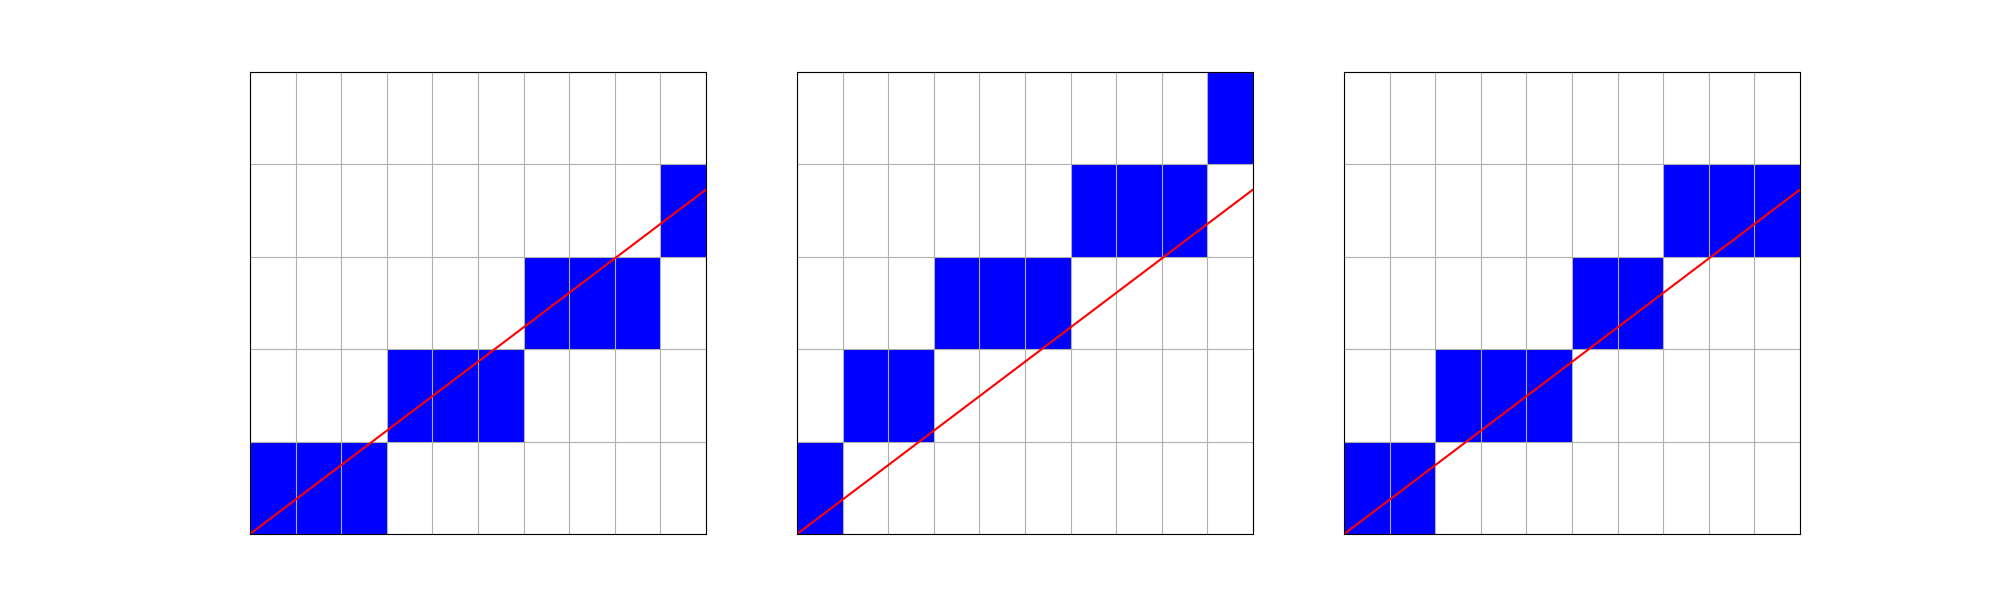
\includegraphics[width=\linewidth]{figures/schanuel_function_approximation}
    \caption{A linear function and three of its approximations}
    \label{fig:the_real_numbers:schanuel_function_approximation}
\end{figure}

Whichever two reasonable approximations one chooses, the following should hold~\cite{Piponi2006}.
\begin{itemize}
    \item When their underlying functions are equal, their difference should be bounded. That is, no two approximations of the same function can differ too much.
    \item When their underlying function are unequal, their difference should be unbounded. That is, two approximations should differ arbitrarily much when the underlying functions are unequal.
\end{itemize}
This induces an equivalence relation on the approximations of functions. Two approximations are regarded the same when their difference is bounded. We will now convert this intuition to mathematical statements. Recall from Definition~\ref{dfn:the_natural_numbers_integers_and_rational_numbers:ordered_semiring_homomorphism} that a homomorphism $f$ preserves addition, that is $f(a+b)=f(a)+f(b)$.
\begin{definition}[Almost homomorphism]
    A function $f:\bbZ\to\bbZ$ is an almost homomorphism if $\{f(a+b)-f(a)-f(b)\mid a\in\bbZ\land b\in\bbZ\}$ is bounded.
\end{definition}
\begin{definition}[Almost equal]
    Almost homomorphisms $f:\bbZ\to\bbZ$ and $g:\bbZ\to\bbZ$ are almost equal if $\{f(a)-g(a)\mid a\in\bbZ\}$ is bounded.
\end{definition}
A function being an almost homomorphism means that it is a reasonable approximation of a linear function. It is almost linear. In particular, we measure the almostness of an almost homomorphism by $S_f=\max\{\vert f(a+b)-f(a)-f(b)\vert\mid a\in\bbZ\land b\in\bbZ\}$.

Note that A'Campo used different, but equivalent, definitions for almost homomorphisms and almost equality. He required that instead of bounded, the sets are finite. While this can be shown to be equivalent, we have not defined finiteness of sets. To avoid this additional overhead we have stated the definitions in terms of boundedness.

This construction has also been given the name ``Eudoxus real numbers'', for example by Arthan in~\cite{Arthan2004}. This is because they can be interpreted within the theory of proportions by Eudoxus. More specifically Definition~5 in Book~5 of Euclid's \textit{Elements} gives rise to this construction. This is precisely the definition that gave rise to the Dedekind real numbers too. See~\cite{Arthan2004} for the details regarding this. We will call them the Schanuel real numbers like we have done for the Dedekind and Cantor real numbers.

We will now mathematically state the relation on the almost homomorphisms. Define the relation $\sim$ on
\begin{equation*}
    \operatorname{AEnd}(\bbZ)\coloneq\{f\in\bbZ^\bbZ\mid f\text{ is an almost homomorphism}\}
\end{equation*}
by
\begin{equation}\label{eqn:the_real_numbers:schanuels_relation_real_numbers}
    f\sim g\iff f\text{ and }g\text{ are almost equal}.
\end{equation}
\begin{lemma}
    The relation $\sim$ as defined in Equation~\eqref{eqn:the_real_numbers:schanuels_relation_real_numbers} is an equivalence relation.
\end{lemma}
\begin{proof}
    Reflexivity is clear as the set $\{0\}$ is definitely bounded. Symmetry follows as any bound for $\{f(a)-g(b)\mid a\in\bbZ\land b\in\bbZ\}$ will also work for $\{-(f(a)-g(b))
    \mid a\in\bbZ\land b\in\bbZ\}$. For transitivity, suppose $f\sim g$ and $g\sim h$. Define $A=\{f(a)-g(b)\mid a\in A\land b\in\bbZ\}$, $B=\{g(b)-h(c)\mid b\in\bbZ\land c\in\bbZ\}$ and $C=\{f(a)-h(c)\mid a\in\bbZ\land c\in\bbZ\}$. Then $C=A+B$. Since $A$ and $B$ are bounded, there exists an $M\in\bbN$ such that for all $a\in A$ we have $\vert a\vert\leq M$ and similarly an $N\in\bbN$ such that for all $b\in B$ we have $\vert b\vert\leq N$. Since $\vert a+b\vert\leq\vert a\vert+\vert b\vert\leq M+N$ we have that $C$ is bounded.
\end{proof}

\begin{definition}[Real numbers]
    Define the set $\bbR_S$ of (Schanuel) real numbers by $\bbR_S\coloneq\operatorname{AEnd}(\bbZ)/{\sim}$.
\end{definition}

\begin{definition}[Addition of real numbers]
    Define addition as the map $\bbR_S\times\bbR_S\to\bbR_S$ defined by
    \begin{equation*}
        [f]+[g]=[f+g].
    \end{equation*}
\end{definition}
It follows that $f+g$ is an almost homomorphism by the proof of transitivity of $\sim$. One should check that this operation is independent of the representative.
\begin{proposition}\label{prp:the_real_numbers:schanuel_abelian_group_real_numbers}
    $(\bbR_S,+)$ is an abelian group.
\end{proposition}
\begin{proof}
    Because addition works pointwise, all properties follow directly by Proposition~\ref{prp:the_natural_numbers_integers_and_rational_numbers:abelian_group_integers}. The identity is the zero function $0:\bbZ\to\bbZ$. The inverse of $[f]\in\bbR_S$ is given by $-[f]\coloneq[-f]$.
\end{proof}

\begin{definition}[Multiplication of real numbers]
    Define multiplication as the map $\bbR_S\times\bbR_S\to\bbR_S$ defined by
    \begin{equation*}
        [f]\cdot[g]=[f\circ g].
    \end{equation*}
\end{definition}
One should verify that the composition of two almost homomorphisms is again an almost homomorphism, and that the resulting equivalence class is independent of the chosen representatives.

Next we will define the order on $\bbR_S$. For this, we will induce an order based on classifying the positive real numbers. Notice that linear functions that have a positive slope, also have a positive function value for $x>0$. This can be translated to almost homomorphisms in terms of boundedness.
\begin{definition}[Order on real numbers]\label{dfn:the_real_numbers:schanuel_order}
    Say $[f]>0$ when $f(\bbN)\cap\bbN$ is unbounded. Define the order on $\bbR_S$ as $[f]\leq[g]$ if $[f]=[g]$ or there exists a positive $[h]\in\bbR_S$ such that $[f]+[h]=[g]$.
\end{definition}
One can verify that positivity of $[f]$ is independent of the representative. We have now defined all operations on the real $\bbR_S$. Before we show that these operations define an ordered field, we will establish a useful representation of the real numbers.
\begin{definition}[Odd function]
    A function $f:\bbZ\to\bbZ$ is odd when $f(-a)=-f(a)$ for all $a\in\bbZ$.
\end{definition}
\begin{lemma}\label{lma:the_real_numbers:homomorphism_equivalent_odd_homomorphism}
    Every almost homomorphism is equivalent to an odd almost homomorphism.
\end{lemma}
\begin{proof}
    Let $f:\bbZ\to\bbZ$ be an almost homomorphism. Define $g:\bbZ\to\bbZ$ by $g(0)=0$, $g(a)=f(a)$ for $a>0$ and $g(a)=-f(-a)$ for $a<0$. Then $g$ is an almost homomorphism and odd. We also have $f\sim g$ as for $a>0$ we have $f(a)-g(a)=f(a)-f(a)=0$. Because $f$ is an almost homomorphism, for $a<0$ we have that $\vert f(a)+f(-a)-f(0)\vert\leq M$ for some $M\in\bbN$. Hence $\vert f(a)+f(-a)\vert$ is bounded.
\end{proof}
By Lemma~\ref{lma:the_real_numbers:homomorphism_equivalent_odd_homomorphism} it follows that for a function $f:\bbZ\to\bbZ$ it suffices to show that $\{f(a+b)-f(a)-f(b)\mid a\in\bbN\land b\in\bbN\}$ is bounded to show it is an almost homomorphism. This lemma can be used to go one step further.
\begin{definition}[Well-adjusted almost homomorphism]
    An almost homomorphism $f:\bbZ\to\bbZ$ is well-adjusted if $\vert f(a+b)-f(a)-f(b)\vert\leq1$ for all $a\in\bbZ$ and $b\in\bbZ$.
\end{definition}
\begin{lemma}[Concentration lemma, Lemma~4 in~\cite{ACampo2003}]\label{lma:the_real_numbers:concentration_lemma}
    Every almost homomorphism is equivalent to a well-adjusted almost homomorphism.
\end{lemma}
Using this lemma, one can obtain the following properties. Let $[f]\in\bbR_S$ be arbitrary. Assume $f$ is well-adjusted.
\begin{enumerate}
    \item For all $a\in\bbZ$ we have $(\vert f(a+1)-f(a)\vert\leq\vert f(1)\vert+1)$.
    \item We have $[f]>0$ if and only if there exists an $a\in\bbZ$ such that $f(a)>1$.
\end{enumerate}
From this lemma, the following result can be proven.
\begin{lemma}[Lemma~5 in~\cite{ACampo2003}]\label{lma:the_real_numbers:almost_homomorphism_each_value_finitely_often}
    Let $f:\bbZ\to\bbZ$ be an almost homomorphism. If $f(\bbZ)$ is unbounded then there exists $b\geq0$ and $B\geq0$ such that the following properties hold.
    \begin{align*}
        & \forall a\in\bbZ\forall n\in\bbN(\vert f(a+n)-f(a)\vert\leq n\cdot b), \\
        & \forall a\in\bbZ\forall n\in\bbN(\vert f(a+n\cdot B)-f(a)\vert\geq n).
    \end{align*}
    Additionally for all $b\in\bbZ$ we have $f(a)=b$ for at most $2\cdot B-1$ different values of $a$.
\end{lemma}
With this, we are in good shape to prove that $\bbR_S$ is an ordered field.
\begin{proposition}\label{prp:the_real_numbers:schanuel_ordered_field_real_numbers}
    $(\bbR_S,+,\cdot,\leq)$ is an ordered field.
\end{proposition}
\begin{proof}
    By Proposition~\ref{prp:the_real_numbers:schanuel_abelian_group_real_numbers} we have that $(\bbR_S,+,\cdot)$ is an abelian group. It remains to show that $(\bbR_S,+,\cdot)$ is a field, that $(\bbR_S,\leq)$ is a total order and that the order is preserved under addition and multiplication. Associativity of $\cdot$ follows because function composition is associative. We define the multiplicative identity as $1\coloneq[\id]$ where $\id:\bbZ\to\bbZ$ is the identity function. Then for all $[f]\in\bbR_S$ we have $[f]\cdot[i]=[f\circ\id]=[f]$.
    \begin{description}
        \item[Commutative.] Let $[f]\in\bbR_S$ and $[g]\in\bbR_S$ be arbitrary. Because the almostness of the almost homomorphisms $f$ and $g$ is bound by $S_f$ and $S_g$ respectively, we obtain the following estimate.
        \begin{align*}
            a\cdot f(g(a))=f(a\cdot g(a))+E_1=f(g(a)\cdot a)+E_1=g(a)\cdot f(a)+E_2+E_1,
        \end{align*}
        where $\vert E_1\vert\leq\vert a\vert S_f$ and $\vert E_2\vert\leq\vert g(a)\vert S_f\leq\vert a\vert(\vert g(1)\vert+S_g)S_f$. By symmetry we obtain a similar estimate for $a\cdot g(f(a))$. We find
        \begin{align*}
            \vert a\cdot f(g(a))-a\cdot g(f(a))\vert & =\vert g(a)\cdot f(a)+E_2+E_1-f(a)\cdot g(a)-E_4-E_3\vert \\
            & =\vert E_2+E_1-E_4-E_3\vert \\
            & \leq\vert a\vert\bigl((\vert g(1)\vert+S_g)S_f+S_f \\
            & +(\vert f(1)\vert+S_f)S_g+S_g\bigr)
        \end{align*}
        and so
        \begin{equation*}
            \vert f(g(a))-g(f(a))\vert\leq S_f(\vert g(1)\vert+S_g+1)+S_g(\vert f(1)\vert+S_f+1).
        \end{equation*}
        We conclude $f\circ g$ and $g\circ f$ are equivalent, and hence $[f]\cdot[g]=[g]\cdot[f]$.
        \item[Inverse.] Let $[f]\in\bbR_S$ with $[f]\neq0$ be arbitrary. By commutativity it suffices to find a right inverse for $[f]$. That is, an almost homomorphism $g$ such that $f\circ g\sim\id$. By Lemma~\ref{lma:the_real_numbers:concentration_lemma} we can assume $f$ is well-adjusted. For any $m\in\bbZ$ we can therefore find $n_m\in\bbZ$ for which $\vert m-f(n_m)\vert\leq\vert f(1)\vert+1$. By well-ordering of $\bbN$ we can take $n_m$ for which $\vert n_m\vert$ is least, and $n_m>0$ when two different integers attain this minimum. This allows us to define the map $g:\bbZ\to\bbZ$ defined by $g(m)=n_m$. We will prove that $g$ is the right inverse of $f$. We will first have to prove $g$ is an almost homomorphism. We have
        \begin{align*}
            \vert f(g(a+b)-g(a)-g(b))\vert & =f(n_{a+b}-n_a-n_b) \\
             & \leq\vert (a+b)-a-b\vert+2+3(\vert f(1)\vert+1) \\
             & =3\vert f(1)\vert+5.
        \end{align*}
        Since $f(\bbZ)$ is unbounded, it then follows by Lemma~\ref{lma:the_real_numbers:almost_homomorphism_each_value_finitely_often} that $\{g(a+b)-g(a)-g(b)\mid a\in\bbZ\land b\in\bbZ\}$ is bounded. We further have $\id\sim f\circ g$ since $\vert m-f(g(m))\vert=\vert m-f(n_m)\vert\leq\vert f(1)\vert+1$, so $\{i(m)-f(g(m))\mid m\in\bbZ\}$ is bounded. We conclude $[f]\cdot[g]=1$.
        \item[Distributive.] Let $[f]\in\bbR_S$, $[g]\in\bbR_S$ and $[h]\in\bbR_S$ be arbitrary. Then $[f]\cdot([g]+[h])=[(g+h)\circ f]=[g\circ f]+[h\circ f]=[f\circ g]+[f\circ h]$.
        \item[Transitive.] Suppose $[f]\leq[g]$ and $[g]\leq[h]$, that is $[g-f]\geq0$ and $h-g\geq0$. We need to show that $[h-f]\geq0$. If $f\sim g$ or $g\sim h$ then the result trivially follows. We may assume that $g-f$ and $h-g$ are well-adjusted. Since $[g-f]>0$ there exists $m\in\bbN\setminus\{0\}$ and $n\in\bbN\setminus\{0\}$ for which $g(m)-f(m)>1$ and $h(n)-g(n)>1$. Then $m\cdot n\geq m$ and $m\cdot n\geq n$ so that $h(m\cdot n)-f(m\cdot n)>2$. Hence $[h-f]>0$.
        \item[Antisymmetric.] Suppose $[f]\leq[g]$ and $[g]\leq[f]$. If $[f]=[g]$ we are done. Else there exists positive $[h_1]\in\bbR_S$ and $[h_2]\in\bbR_S$ such that $[f+h_1]=[g]$ and $[g+h_2]=[f]$. Then $[g+h_2+h_1]=[g]$, so $[h_1]=-[h_2]$. This must mean $[h_1]=[h_2]=0$ as otherwise either $[h_1]$ or $[h_2]$ would be negative. Hence $[f]=[g]$.
        \item[Strongly connected.] Let $[f]\in\bbR_S$ and $[g]\in\bbR_S$ be arbitrary. Assume $f-g$ is well-adjusted. If $f(a)-g(a)\in\{-1,0,1\}$ for all $a\in\bbZ$, then $f=g$. If not, then by the contrapositive there exists $a\in\bbZ$ for which $f(a)-g(a)<-1$ or $f(a)-g(a)>1$. If $f(a)-g(a)<-1$ then $g(a)-f(a)>1$, so $g-f>0$. If $f(a)-g(a)>1$ then $f-g>0$.
        \item[OR1.] Let $[f]\in\bbR_S$, $[g]\in\bbR_S$ and $[h]\in\bbR_S$ be arbitrary. If $[f]=[g]$ the result follows trivially. Suppose $[f]<[g]$. Then there exists a positive $[j]\in\bbR_S$ so that $[f]+[j]=[g]$. Then $[f]+[h]+[j]=[g]+[h]$, so $[f]+[h]<[g]+[h]$.
        \item[OR2.] Let $[f]\in\bbR_S$, $[g]\in\bbR_S$ and $[h]\in\bbR_S$ with $[h]>0$ be arbitrary. If $[f]=[g]$ the result follows trivially. Else there exists a positive $[j]\in\bbR_S$ such that $[f]+[j]=[g]$. Hence $[f]\cdot[h]+[j]\cdot[h]=[g]\cdot[h]$ by distributivity. Since $[j]\cdot[h]>0$, we find $[f]\cdot[h]<[g]\cdot[h]$.
    \end{description}
\end{proof}
Since this construction did not give rise to a natural new notion of completeness, A'Campo proved that $\bbR_S$ is Dedekind-complete. In particular, he proved the equivalent statement to Dedekind-completeness formulated in Proposition~\ref{prp:the_real_numbers:characterisation_dedekind_complete}. That is, each bounded above subset of $\bbR_S$ has a supremum.
\begin{proposition}\label{prp:the_real_numbers:schanuel_R_dedekind_complete}
    $(\bbR_S,+,\cdot,\leq)$ is an ordered Dedekind-complete field.
\end{proposition}
See~\cite{ACampo2003} for the proof. Note that we have skipped over the rational numbers. Since they are still useful to know, we want to define them anyways. Therefore instead of defining an embedding, we will extract the rational numbers from the real numbers. Note that for integers $a$ and $b$, the rational number ``$a/b$'' is the solution of $b\cdot x=a$.
\begin{definition}[Rational numbers]
    Define the rational numbers $\bbQ_{\bbR_S}$ by
    \begin{equation*}
        \bbQ_{\bbR_S}\coloneq\{[f]\in\bbR_S\mid\exists a\in\bbZ\exists b\in\bbN\setminus\{0\}\forall c\in\bbZ(f(c)=\min\{n\in\bbN\mid b\cdot n\geq a\cdot c\})\},
    \end{equation*}
    where $f$ is extended oddly.
\end{definition}
It can be shown that $\bbQ_{\bbR_S}$ is isomorphic to $\bbQ$. The isomorphism would be $f:\bbQ\to\bbQ_{\bbR_S}$ given by 
\begin{equation*}
    f(a/b)=[(g:\bbZ\to\bbZ,g(c)=\min\{n\in\bbN\mid b\cdot n\geq a\cdot c\})].
\end{equation*}
This defines the rational numbers explicitly. Note that we already knew that the rational numbers exist in $\bbR_S$ by Theorem~\ref{thm:the_natural_numbers_integers_and_rational_numbers:Q_smallest_ordered_field}.

\section{Uniqueness of \texorpdfstring{$\bbR$}{ℝ}}\label{sec:the_real_numbers:uniqueness_of_R}
We have constructed three sets we all called the real numbers: $\bbR_D$, $\bbR_C$ and $\bbR_S$. Since we gave them the same name, it would also be favourable that they are the same mathematically. To do that, we will show that the properties each construction has are interchangeable, so that each set satisfies all the same properties. After that, we will show that any set that has these properties, is essentially the same set. This proves the structural equality of our three sets, and the uniqueness of the real numbers in general.

We asserted earlier that Cauchy-completeness is a weaker property than Dedekind-completeness. The missing requirement is the Archimedean property. We will now prove this.
\begin{theorem}\label{thm:the_real_numbers:equivalence_cauchy_dedekind_completeness}
    Let $\bbK$ be an ordered field. Then $\bbK$ is a Cauchy-complete Archi\-medean field if and only if $\bbK$ is a Dedekind-complete field.
\end{theorem}
\begin{proof}
    For the forward direction suppose $\bbK$ is an ordered Cauchy-complete Archimedean field. Let $A$ be a Dedekind cut of $\bbK$. We want to construct a Cauchy sequence that approaches the cutting point of $A$. Since the sequence is then convergent by Cauchy-completeness, we can prove the Dedekind cut $A$ is then produced by some $x\in\bbK$, where $x$ is the limit of the sequence.

    Start by taking $x_0=a$ for any $a\in A$. For $n\in\bbN$ define $x_{n+1}=x_n+k/2^n$ where $k$ is the largest $k\in\bbN$ for which $x_n+k/2^n\in A$. We can do this as by the Archimedean property there exists a $l$ such that $x_n+l/2^n$ is larger than any $b\in\bbK\setminus A$. By the well-ordering of $\bbN$ we can then take the minimal $k+1$ for which $x_n+(k+1)/2^n$ is in $\bbK\setminus A$ and less than or equal to $x_n+l/2^n$. Then $k$ is the largest $k\in\bbN$ such that $x_n+k/2^n\in A$.

    To see that $(x_n)$ is Cauchy, by way of contradiction suppose for $m\leq n$ that $x_n>x_m+1/2^{m-1}$. Since $x_n\in A$, we also have $x_m+1/2^{m-1}\in A$. But that means $x_m+1/2^{m-1}=x_{m-1}+(k_{m-1}+1)/2^{m-1}\in A$, violating maximality of $k_{m-1}$. Hence $\vert x_m-x_n\vert\leq1/2^{m-1}$, so $(x_n)$ is Cauchy. Therefore $x_n\to x$ for some $x\in\bbK$. We claim that $A$ is the Dedekind cut produced by $x$; that is $A=\{a\in\bbK\mid a<x\}$. We will first show $\{a\in\bbK\mid a<x\}\subseteq A$ by contrapositive. Suppose $a\notin A$. Then $a\geq x_n$ for all $n\in\bbN$. Hence $a\geq x$. To show $A\subseteq\{a\in\bbK\mid a<x\}$, let $a\in A$ be arbitrary and by way of contradiction suppose $a\geq x$. Then $a\geq x\geq x_n$ for all $n\in\bbN$. Since $A$ contains no greatest element, there is a $b\in A$ such that $b>a$. Then by the Archimedean property we can find an $n\in\bbN$ for which $a+1/2^n<b$. Since $x_{n+1}+1/2^n\notin A$ we have $b<x_{n+1}+1/2^n$ so that $b-1/2^n<x_{n+1}\leq a$, a contradiction. We conclude $\bbK$ is Dedekind-complete.

    For the converse suppose $\bbK$ is an ordered Dedekind-complete field. To prove $\bbK$ is Archimedean, by way of contradiction suppose there exists an $x\in\bbK$ such that for all $n\in\bbN$ we have $n<x$. Then $\bbN$ is bounded above by $x$, so by Proposition~\ref{prp:the_real_numbers:characterisation_dedekind_complete} there exists a supremum $S$ of $\bbN$. Then $S-1$ is not an upper bound, so there exists an $m\in\bbN$ such that $m>S-1$, hence $S<m+1$. But $m+1\in\bbN$, contradicting that $S$ is an upper bound. Hence $\bbK$ is Archimedean.

    Next, let $(x_n):\bbN\to\bbK$ be a Cauchy sequence. To show $(x_n)$ is convergent we need to find a candidate limit. Because we have Dedekind-completeness, perhaps a natural idea is to consider the suprema of the elements of $(x_n)$. For all $n\in\bbN$ define $A_n=\{x_m\in\bbK\mid m\geq n\}$. Since $A_n$ is bounded because Cauchy sequences are, by Proposition~\ref{prp:the_real_numbers:characterisation_dedekind_complete} it has a supremum $S_n$. Then $(S_n)$ is a bounded decreasing sequence. We will prove $(S_n)$ is convergent. Notice that $(-S_n)$ is a bounded increasing sequence, so that we can define $-S$ to be the supremum of $\{-S_n\in\bbK\mid n\in\bbN\}$. Then since $-S$ is the supremum, for every $\epsilon>0$ there exists an $N\in\bbN$ such that $-S_N>-S-\epsilon$. Now because $(-S_N)$ is increasing, for $n\geq N$ we have
    \begin{equation*}
        \vert-S-(-S_n)\vert=-S-(-S_n)\leq-S-(-S_N)<\epsilon.
    \end{equation*}
    We conclude $-S_n\to-S$ and therefore also $S_n\to S$. Define $B_n=\{-x_m\in\bbK\mid m\geq n\}$. Since $B_n$ is also bounded, it has a supremum $T_n$. By a similar argument $T_n\to T$ where $T$ is the supremum of $\{T_n\in\bbK\mid n\in\bbN\}$. We will show $S=T$. Let $\epsilon>0$ be arbitrary. Take $N\in\bbN$ to be maximum of the $N$ necessary for the Cauchy property, such that $S_N>S-\epsilon$ and such that $T_N<T+\epsilon$. Then
    \begin{align*}
        \vert S-T\vert & =\vert S-S_N+S_N+T_N-T_N-T\vert \\
        & \leq\vert S-S_N\vert+\vert S_N-T_N\vert+\vert T-T_N\vert \\
        & <\epsilon+\epsilon+\epsilon=3\epsilon.
    \end{align*}
    Since this holds for all $\epsilon>0$, we must have $S=T$. We will now show $x_n\to S$. Let $\epsilon>0$ be arbitrary. Take $N\in\bbN$ such that for $n\geq N$ we have $x_n>S-\epsilon$ and $x_n<S+\epsilon$. Then $S-\epsilon<x_n<S+\epsilon$, so
    \begin{equation*}
        -\epsilon<x_n-S<\epsilon\implies\vert x_n-S\vert<\epsilon.
    \end{equation*}
    We conclude $x_n\to S$.
\end{proof}
We conclude by the above theorem, and by Propositions~\ref{prp:the_real_numbers:dedekind_R_dedekind_complete},\linebreak\ref{prp:the_real_numbers:cantor_R_cauchy_complete_archimedean}~and~\ref{prp:the_real_numbers:schanuel_R_dedekind_complete} that all of $\bbR_D$, $\bbR_C$ and $\bbR_S$ are Dedekind-complete, Cauchy-complete and satisfy the Archimedean property. We will now show that any ordered field with these properties is essentially the same field. Like we have done thus far, we want to reuse the definition of the function $\varphi$ we used in the proof of Theorem~\ref{thm:the_natural_numbers_integers_and_rational_numbers:Q_smallest_ordered_field}. There we were able to induce a definition for $\varphi$ for the integers based on the natural numbers, and for the rational numbers based on the integers. However, it is not immediately clear how one would induce a definition for the real numbers based on the rational numbers.

We saw that Cauchy sequences allowed us to expose the real numbers from the rational numbers. Given that real Cauchy sequences are now also convergent, perhaps we can define $\varphi$ for the real numbers by constructing rational sequences that converge to the real numbers. The image of the sequence under $\varphi$ would then also be a rational sequence. We would then want this image sequence to converge as well, so to induce a definition for the real numbers. We want this to be the case in the codomain of $\varphi$ as well. That is, now that we can define $\varphi$ for the real numbers, we want to be sure that with this we can reach all numbers in the codomain. Informally put, we want to be able to approximate the values in the codomain by the rational numbers that exist in the codomain. The following proposition assures that this is the case for any Archimedean field.
\begin{proposition}[$\bbQ$ is dense in any ordered Archimedean field]\label{prp:the_real_numbers:Q_dense_in_ordered_archimedean_field}
    Let $(R,+,\linebreak\cdot,\leq)$ be an ordered Archimedean field. By Theorem~\ref{thm:the_natural_numbers_integers_and_rational_numbers:Q_smallest_ordered_field} there exists a copy of $\bbQ$ in $R$. Then for any $x\in R$ and $y\in R$ with $x<y$ there exists a $q\in\bbQ$ such that $x<q<y$.
\end{proposition}
\begin{proof}
    By the Archimedean property there exists an $n\in\bbN$ such that $n>1/(y-x)$. Rewriting yields $n\cdot x+1<n\cdot y$. It can be verified that again by the Archimedean property, along with the well-ordering of $\bbN$, there exists a minimal $m\in\bbZ$ such that $n\cdot x<m$. Because this $m$ is minimal, we have $m-1\leq n\cdot x<m$. Thus $n\cdot x<m\leq n\cdot x+1<n\cdot y$. We conclude $n\cdot x<m<n\cdot y$ so that $x<m/n<y$.
\end{proof}
With this, we can now turn to proving the uniqueness of the real numbers. It was Huntington who in 1903 first characterised the real numbers using a set of properties they should satisfy~\cite{Huntington1903}. We will state the uniqueness in terms of Cauchy-completeness and the Archimedean property. We will do this because we will use Proposition~\ref{prp:the_real_numbers:Q_dense_in_ordered_archimedean_field} and Cauchy-completeness intensively. Of course, by Theorem~\ref{thm:the_real_numbers:equivalence_cauchy_dedekind_completeness} this can be equivalently stated in terms of Dedekind-completeness.
\begin{theorem}[Uniqueness of $\bbR$]\label{thm:the_real_numbers:uniqueness_R}
    $(\bbR,+,\cdot,\leq)$ is the unique ordered Cauchy-complete Archimedean field.
\end{theorem}
\begin{proof}
    Let $\bbR_C$ be the Cantor real numbers. Let $R$ be an ordered Cauchy-complete Archimedean field. We will start to define $\varphi:\bbR_C\to R$ as in the proof of Theorem~\ref{thm:the_natural_numbers_integers_and_rational_numbers:Q_smallest_ordered_field}. Briefly put, define $\varphi(0_{\bbR_C})=0_R$ and $\varphi(q+1_{\bbR_C})=\varphi(q)+1_R$. We then extended this to the integers by $\varphi(-q)=-\varphi(q)$. In the same way we extended $\varphi$ to the rational numbers by $\varphi(p\cdot q^{-1})=\varphi(p)\cdot\varphi(q)^{-1}$. This yielded an ordered field isomorphism with respect to rational number addition, multiplication and order. To extend $\varphi$ to all of its domain, we will extend $\varphi$ using sequences. Notice that $\varphi(\bbQ)$ is isomorphic to $\bbQ$ by Theorem~\ref{thm:the_natural_numbers_integers_and_rational_numbers:Q_smallest_ordered_field}. Let $(x_n):\bbN\to\bbQ$ be a Cauchy (hence convergent) sequence, so $x_n\to x$ for some $x\in\bbR_C$. We will show $(\varphi(x_n))$ is Cauchy too. Let $\epsilon>0_\bbQ$ be arbitrary. Because $(x_n)$ is Cauchy, we can take $N$ such that for all $m\geq N$ and $n\geq N$ we have $\vert x_m-x_n\vert<\varphi^{-1}(\epsilon)$. Then $-\varphi^{-1}(\epsilon)<x_m-x_n<\varphi^{-1}(\epsilon)$ so that $-\epsilon<\varphi(x_m)-\varphi(x_n)<\epsilon$ because $\varphi$ is an ordered field isomorphism on $\bbQ$. Hence $\vert\varphi(x_m)-\varphi(x_n)\vert<\epsilon$. We conclude $(\varphi(x_n))$ as a function $\bbN\to\bbQ$ is Cauchy. It remains to verify it is Cauchy as a function $\bbN\to R$ as well. For this we use that $\bbQ$ is dense in $R$ by Proposition~\ref{prp:the_real_numbers:Q_dense_in_ordered_archimedean_field}. Then for any $\epsilon>0_R$ we can find a smaller positive $\epsilon\in\bbQ$, proving $(\varphi(x_n))$ is Cauchy as a function $\bbN\to R$. We therefore have $\varphi(x_n)\to y$ for some $y\in R$. We define $\varphi(x)=y$. Since every real number can be approximated by rational Cauchy sequences, this defines $\varphi$ for all real numbers. One should verify this extension is well-defined. That is, the mapping of $\varphi$ should be independent of the sequence chosen. This follows by showing that when $x_n\to0_{\bbR_C}$ we also have $\varphi(x_n)\to0_R$. As this follows reasoning identical to what we did above, we will not do it again. We will turn to showing that $\varphi$ defines an ordered field isomorphism.
    \begin{description}
        \item[Field homomorphism.] Clearly $\varphi(0_{\bbR_C})=0_R$ and $\varphi(1_{\bbR_C})=1_R$. Let $x\in\bbR_C$ and $y\in\bbR_C$ be arbitrary. There exists rational sequences $(x_n):\bbN\to\bbQ$ and $(y_n):\bbN\to\bbQ$ such that $x_n\to x$ and $y_n\to y$. Then $\varphi(x_n+y_n)\to\varphi(x+y)$ and $\varphi(x_n+y_n)=\varphi(x_n)+\varphi(y_n)\to x+y$. Since limits are unique, we have $\varphi(x+y)=\varphi(x)+\varphi(y)$.

        Similarly $\varphi(x_n\cdot y_n)\to\varphi(x\cdot y)$ and $\varphi(x_n\cdot y_n)=\varphi(x_n)\cdot\varphi(y_n)\to\varphi(x)\cdot\varphi(y)$. Hence $\varphi(x\cdot y)=\varphi(x)\cdot\varphi(y)$.
        \item[Injective.] Injectivity follows from the fact that $\varphi$ is a field homomorphism. Indeed, suppose $\varphi(x)=\varphi(y)$ for some $x\in\bbR_C$ and $y\in\bbR_C$. We want to show that $x=y$. We have $\varphi(x-y)=0_R$. Let $z=x-y$. By way of contradiction, suppose $z\neq0_{\bbR_C}$. Then $\varphi(z)\cdot\varphi(z^{-1})=\varphi(1_{\bbR_C})=1_R$. Since $\varphi(z)=0_R$ it follows that $0_R\cdot\varphi(z^{-1})=1_R$, a contradiction.
        \item[Order homomorphism.] Let $x\in\bbR_C$ and $y\in\bbR_C$ with $x\leq y$ be arbitrary. There exists rational Cauchy sequences $(x_n):\bbN\to\bbQ$ and $(y_n):\bbN\to\bbQ$ such that $x_n\to x$, $y_n\to y$ and additionally with the property that $x_n\leq y_n$ for all $n\in\bbN$. Then $\varphi(x_n)\leq\varphi(y_n)$ for all $n\in\bbN$ so that $\varphi(x)\leq\varphi(y)$.
        \item[Surjective.] Let $y\in R$ be arbitrary. We will prove there exists a sequence $(y_n):\bbN\to\bbQ$ such that $y_n\to y$. Because $\bbQ$ is dense in $R$, for all $n\in\bbN$ we can take $y_n\in\bbQ$ such that $y-1/n<y_n<y+1/n$. Let $\epsilon>0_R$ be arbitrary. By the Archimedean property we can find an $N\in\bbN$ such that $1/N<\epsilon$. Then for $n\geq N$ we find $\vert y_n-y\vert<1/n\leq1/N<\epsilon$. We conclude $y_n\to y$. The restriction of $\varphi$ to $\varphi\vert_\bbQ:\bbQ\to\varphi(\bbQ)$ is an isomorphism so by bijectivity of $\varphi\vert_\bbQ$ we can define the sequence $(x_n):\bbN\to\bbQ$ by $x_n=\varphi\vert_\bbQ^{-1}(y_n)$. By similar reasoning as above, we find that $(x_n)$ is Cauchy, and Cauchy as a function $\bbN\to R$ as well. It therefore converges to some $x\in\bbR_C$. For this $x$ we have $\varphi(x)=y$.
    \end{description}
\end{proof}
We have done it; we have proven the existence and uniqueness of the real numbers. We are now free to write $\bbR$ without any subscript, without the need for specifying its precise set-theoretic definition, and without the need for specifying its properties; as we have been doing all our lives.

\section{Comparison of the constructions}\label{sec:the_real_numbers:comparison_of_the_constructions}
In this section we will take a step back and remove our blindfolds for knowledge exterior to what we have established so far. That means that we will assume knowledge of other fields in mathematics to give a more informed overview of the constructions.

Before comparing the constructions themselves, we will look at their structure in terms of sets, see also~\cite{Borovik2012}. Note that we built the rational numbers as equivalence classes of pairs of integers. Let $\alpha$ extract these equivalence classes from the pairs. That is $\bbQ=(\bbZ\times\bbZ)_\alpha$. We find the following compositions of the real numbers.
\begin{align*}
    \bbR_D & =\left(\mathcal{P}\left((\bbZ\times\bbZ)_\alpha\right)\right)_\delta, \\
    \bbR_C & =(\bbN\to(\bbZ\times\bbZ)_\alpha)_\gamma, \\
    \bbR_S & =(\bbZ\to\bbZ)_\sigma,
\end{align*}
where $\delta$ extracts the Dedekind cuts, $\gamma$ the Cauchy sequences and $\sigma$ the almost homomorphisms. We see that purely constructionally, the Schanuel real numbers are the most simple. Where the other constructions have two restrictions, the Schanuel real numbers have only one.

Let us now consider Dedekind's construction. In his construction, each real number is represented by a single Dedekind cut. This is advantageous, as it makes any function (relation) defined on them almost automatically univalent. It only would only remain to show it is total. 

Dedekind's construction also generalises well to general ordered sets. In fact, the order need not satisfy strongly connectedness, in which case it is called a partial order. This generalised completion is known as the Dedekind-MacNeille completion, and works as follows. Let $(S,\leq)$ be a partial order. For $A\subseteq S$ define $\upp(A)=\{s\in S\mid\forall a\in A(s\geq a)\}$. Then $\upp(A)$ are the upper bounds of $A$. Similarly define the lower bounds of $A$ as $\low(A)=\{s\in S\mid\forall a\in A(s\leq a)\}$. A cut of $S$ is then a pair $(A,B)$ for which $\upp(A)=B$ and $\low(B)=A$. In this case one also has $\low(\upp(A))=A$, so $(A,\upp(A))$ is a cut. Hence similar to Dedekind cuts, one can focus only on the set $A$. Then the sets of cuts of $S$ is the completion of $S$. Note that applying this completion to the rational numbers does not result in the real numbers; it results in the extended real numbers. These are the real numbers along with two elements assuming the roles of negative and positive infinity. This is because Dedekind cuts required $A\neq\varnothing$ and $A\neq\bbQ$, whereas this generalised completion does not require that. The cut $A=\varnothing$ behaves like negative infinity, the cut $A=\bbQ$ behaves like positive infinity.

Contrary to Dedekind real numbers, Cantor real numbers are represented by equivalence classes. Since operations on equivalence classes are defined in terms of their representatives, it is often necessary to verify the operation (relation) is both total and univalent. While this is often readily done, sometimes it is not immediately clear. For example, in general the reciprocal of a Cauchy sequence is not Cauchy. Only because we could cherry-pick the representatives, we were able to make this work.

Similar to Dedekind's construction, Cantor's construction can be easily generalised. Let $X$ be a set and let $d:(X\times X)\to\bbR$ be a function. Then $(X,d)$ is a metric space\footnote{Even more generally, one can consider Cauchy filters in a uniform space. See~\cite{Kelley1975} for more information.} when for all $x\in X$, $y\in X$ and $z\in X$ one has
\begin{itemize}
    \item $d(x,y)\geq0$,
    \item $d(x,y)=0\iff x=y$,
    \item $d(x,y)=d(y,x)$,
    \item $d(x,y)\leq d(x,z)+d(z,y)$.
\end{itemize}
Cauchy sequences can then be defined as sequences for which $d(x_m,x_n)$ gets arbitrarily small for large enough $m\in\bbN$ and $n\in\bbN$. The Cauchy-completion of $X$ is then the set of equivalent Cauchy sequences, where two Cauchy sequences are equivalent when their difference converges to zero. When $X$ additionally is an ordered abelian group, it induces the metric defined by $d(x,y)=\vert y-x\vert$. This metric is precisely the metric we used for the construction of the Cantor real numbers.

Schanuel's construction also relied on equivalence classes, making operations on his real numbers subject to a proof of well-definedness. Though as with Cantor's construction, these are usually not too difficult. Contrary to Cantor's construction though, no assumption on the representative has to be done. All almost homomorphisms remain almost homomorphisms under addition and multiplication.

Schanuel's construction skips over the rational numbers, and therefore avoids all proofs related to them. However, one may object that the rational numbers are to be constructed at some point anyway, because of their usefulness in many occasions. Frankly without them, there is no such thing as rational and irrational numbers. However, Theorem~\ref{thm:the_natural_numbers_integers_and_rational_numbers:Q_smallest_ordered_field} asserts that $\bbQ$ must exist in $\bbR_S$, which is sufficient to know for most cases. If explicit representations of rational numbers in $\bbR_S$ are sought after, we saw that one can construct $\bbQ$ as a subfield of $\bbR_S$. It would have to be shown first that they are indeed isomorphic to $\bbQ$, though.

\section{Further research}\label{sec:the_real_numbers:further_research}
Given that completeness characterised the real numbers, one may wonder wheth\-er there exists a notion of completeness that the real numbers lack. One direction to explore is that of non-Archimedean ordered fields. These include number systems like the surreal~\cite{Conway1976} and hyperreal~\cite{Goldblatt1998} numbers. These are number systems that contain infinitely small and infinitely large numbers, which the real numbers certainly do not. However, one should wonder in what sense these number systems are actually more complete than the real numbers. They are, for example, still not closed under inversion; infinity (``$1/0$'') remains not a number. It turns out that the surreal numbers are ``saturated''~\cite{Michael1963}. The saturation property mandates that for any two subsets\footnote{Note that the surreal numbers are too large to form a set, they form a proper class. However the saturation property only applies to subsets.} $A$ and $B$ of surreal numbers such that every element of $A$ is less than every element of $B$, there exists a surreal number larger than all elements of $A$ and smaller than all elements of $B$. This fails in the real numbers: take any Dedekind cut. Note that the saturation property is a stronger property than Dedekind-completeness.

Related to the surreal and hyperreal numbers are the extended real numbers. These add two quantities ($\infty$ and $-\infty$) to the real numbers that behave like positive and negative infinity. For example one would have $\infty+a=\infty$ for all $a\in\bbR$. Contrary to the surreal and hyperreal numbers, the extended real numbers are closed under inversion. Furthermore, as we alluded to before, the Dedekind-MacNeille completion of the rational numbers yields the extended real numbers. In these senses it would make them more complete. They are also ``topologically compact''; every subset has a supremum. They however no longer form a field. Even worse, they satisfy none of the properties of a field. This is because expressions like ``$\infty-\infty$'' are usually left undefined. The extended real numbers are used in particular in measure theory, where sets are allowed to have infinite measure, functions are allowed to attain infinity and integrals may evaluate to infinity~\cite{Veraar2022}.

Another direction one might venture is that of complex numbers, quaternions, octonions and further\footnote{They can be indefinitely extended using the Cayley-Dickson construction~\cite{Dickson1919}.}. Landau was likely the first to fully describe the construction of the natural numbers all the way to the complex numbers~\cite{Landau1930}. As far as completeness goes, the complex numbers are the most interesting. They satisfy ``algebraic closure'', meaning that any (nonconstant) polynomial has a root in the complex numbers. This fails in the real numbers: consider the function $f:\bbR\to\bbR$ defined by $f(x)=x\cdot x+1$. Beyond the complex numbers it is unclear whether they satisfy any reasonable notion of completeness that the complex numbers do not satisfy. The octonions and further are interesting mostly for other reasons.

It is in general hard to define what a completion or completeness property is or would have to be. If anything, they are classified by the following principle: the space achieved by a completion must be complete with respect to the completeness property the space was completed with. For instance, the Dedekind real numbers are Dedekind-complete and the Cantor real numbers are Cauchy-complete.

Note that all the completions we discussed lost properties the real numbers enjoyed. The surreal numbers are no longer Archimedean, the extended real numbers no longer form a field and the complex numbers can no longer be equipped with an order such that it becomes an ordered field. It seems in this sense the real numbers are at some sort of maximal structure. If one tries to go any higher, the foundation one stands on will lower.
\end{document}
